\documentclass{beamer}
\usetheme{Madrid}
\usecolortheme{default}

\usepackage{amsmath}
\usepackage{booktabs}
\usepackage{array}
\usepackage{pgfplots}
\usepackage{tikz}
\pgfplotsset{compat=1.18}
\usetikzlibrary{patterns,calc,shapes.geometric,arrows.meta,positioning}
\pgfplotsset{
    beamer axis/.style={
        width=0.92\textwidth,
        height=5.8cm,
        grid=major,
        grid style={line width=0.3pt, draw=gray!30},
        title style={font=\small\bfseries},
        label style={font=\footnotesize},
        tick label style={font=\scriptsize},
        legend style={font=\scriptsize},
    }
}

% ---- Title info ----------------------------------------------------------------
\title[Climate Risk \& ECL]{Modeling Physical Climate Risk in IFRS 9 ECL Frameworks:\\
A Two-Regime Markov-Switching Approach to Credit Migration\\
in Zimbabwe's Microfinance Sector}
\subtitle{Under IFRS 9 Compliance}
\author{Kuwana Tadiwanaishe J}
\institute{HIT}
\date{}

\newcommand{\ts}{\footnotesize}

\begin{document}

\frame{\titlepage}

% ============================================================
\begin{frame}
    \frametitle{Presentation Outline}
    \tableofcontents[hideallsubsections]
\end{frame}

% ============================================================
\section{Chapter 1: Introduction}

\begin{frame}
    \frametitle{Background \& Research Gap}
    \begin{columns}[T]
    \column{0.50\textwidth}
    \begin{alertblock}{Zimbabwe's Exposure}
    \small
    \begin{itemize}
        \item 42\% of MFI clients are smallholder farmers
        \item RBZ Portfolio-at-Risk: \textbf{18.7\%} --- 3$\times$ the prudential limit
        \item Drought drives \textit{covariant} defaults across entire portfolios
        \item IFRS 9 mandates \textbf{forward-looking} ECL --- static models fail
    \end{itemize}
    \end{alertblock}
    \vspace{0.3em}
    \begin{block}{Gap}
    \small No exogenous, climate-driven regime-switching ECL model exists for Zimbabwean MFI credit migration.
    \end{block}
    \column{0.46\textwidth}
    \begin{center}
    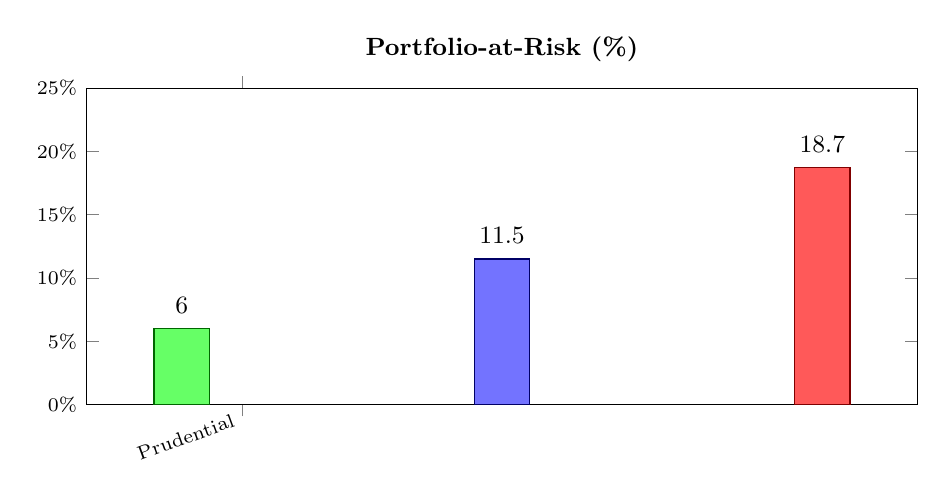
\begin{tikzpicture}
    \begin{axis}[
        width=\linewidth, height=5.6cm,
        ybar, bar width=20pt,
        title={Portfolio-at-Risk (\%)},
        title style={font=\small\bfseries},
        symbolic x coords={Prudential,Static ECL,Actual RBZ},
        xtick=data,
        xticklabel style={font=\scriptsize, rotate=20, anchor=east},
        ymin=0, ymax=25,
        ytick={0,5,10,15,20,25},
        yticklabel={\pgfmathprintnumber{\tick}\%},
        tick label style={font=\scriptsize},
        nodes near coords,
        every node near coord/.append style={font=\small, yshift=2pt},
        enlarge x limits=0.3,
    ]
    \addplot[fill=green!60, draw=green!40!black] coordinates {(Prudential,6)};
    \addplot[fill=blue!55,  draw=blue!40!black]  coordinates {(Static ECL,11.5)};
    \addplot[fill=red!65,   draw=red!50!black]   coordinates {(Actual RBZ,18.7)};
    \end{axis}
    \end{tikzpicture}
    \end{center}
    \end{columns}
\end{frame}

\begin{frame}
    \frametitle{Objectives \& Research Questions}
    \begin{columns}[T]
    \column{0.50\textwidth}
    \textbf{Objectives}
    \begin{enumerate}\small
        \item Classify 2014--2024 into Normal / Drought-Stress regimes using SPEI-3.
        \item Estimate $\hat{M}_{\text{normal}}$ and $\hat{M}_{\text{stress}}$ via MLE.
        \item Validate two-regime structure via LRT and out-of-sample discrimination.
        \item Produce climate-adjusted ECL under four IFRS 9 scenarios.
    \end{enumerate}
    \column{0.46\textwidth}
    \textbf{Key Questions}
    \begin{enumerate}\small
        \item Can SPEI statistically distinguish Normal from Drought-Stress credit regimes?
        \item How different are $\hat{M}_{\text{normal}}$ and $\hat{M}_{\text{stress}}$?
        \item Does regime-switching improve out-of-sample ECL accuracy?
        \item By how much does the static model under-provision under IFRS 9?
    \end{enumerate}
    \end{columns}
\end{frame}

% ============================================================
\section{Literature Review}

\begin{frame}
    \frametitle{Theoretical Pillars \& Literature Gap}
    \begin{center}
    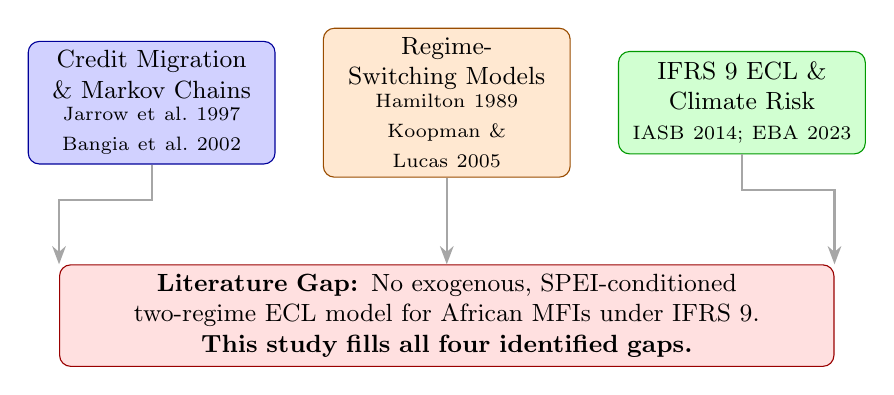
\begin{tikzpicture}[
        boxa/.style={rectangle, rounded corners=4pt, draw=blue!60!black,
                     fill=blue!18, text width=2.9cm, align=center,
                     minimum height=1.3cm, font=\small},
        boxb/.style={rectangle, rounded corners=4pt, draw=orange!60!black,
                     fill=orange!18, text width=2.9cm, align=center,
                     minimum height=1.3cm, font=\small},
        boxc/.style={rectangle, rounded corners=4pt, draw=green!60!black,
                     fill=green!18, text width=2.9cm, align=center,
                     minimum height=1.3cm, font=\small},
        arr/.style={-{Stealth}, thick, gray!70}]
        \node[boxa] (cm)   {Credit Migration \& Markov Chains\\{\scriptsize Jarrow et al.\ 1997\\Bangia et al.\ 2002}};
        \node[boxb, right=0.6cm of cm] (rs)
            {Regime-Switching Models\\{\scriptsize Hamilton 1989\\Koopman \& Lucas 2005}};
        \node[boxc, right=0.6cm of rs] (ifrs)
            {IFRS 9 ECL \&\\Climate Risk\\{\scriptsize IASB 2014; EBA 2023}};
        \node[rectangle, rounded corners=4pt, draw=red!60!black, fill=red!12,
              text width=9.6cm, align=center, minimum height=1.1cm, font=\small,
              below=1.1cm of rs] (gap)
            {\textbf{Literature Gap:} No exogenous, SPEI-conditioned two-regime ECL model for African MFIs under IFRS 9.\\
             \textbf{This study fills all four identified gaps.}};
        \draw[arr] (cm.south)   -- ++(0,-0.45) -| (gap.north west);
        \draw[arr] (rs.south)   -- (gap.north);
        \draw[arr] (ifrs.south) -- ++(0,-0.45) -| (gap.north east);
    \end{tikzpicture}
    \end{center}
\end{frame}

% ============================================================
\section{Chapter 3: Research Methodology}

\begin{frame}
    \frametitle{Methodology Pipeline}
    \begin{center}
    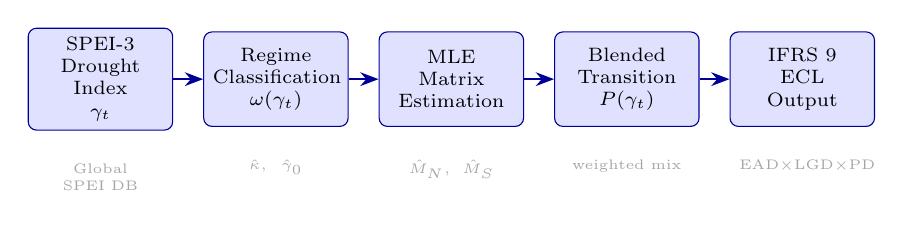
\begin{tikzpicture}[
        stage/.style={rectangle, rounded corners=3pt, draw=blue!60!black,
                      fill=blue!12, text width=1.6cm, align=center,
                      minimum height=1.2cm, font=\scriptsize},
        arr/.style={-{Stealth}, thick, blue!60!black},
        lbl/.style={font=\tiny, text=gray!70, align=center, text width=1.6cm}]
        \node[stage] (spei)  {SPEI-3\\Drought Index\\$\gamma_t$};
        \node[stage, right=0.38cm of spei]  (reg)   {Regime\\Classification\\$\omega(\gamma_t)$};
        \node[stage, right=0.38cm of reg]   (mle)   {MLE\\Matrix\\Estimation};
        \node[stage, right=0.38cm of mle]   (blend) {Blended\\Transition\\$P(\gamma_t)$};
        \node[stage, right=0.38cm of blend] (ecl)   {IFRS 9\\ECL\\Output};
        \draw[arr] (spei) -- (reg);
        \draw[arr] (reg)  -- (mle);
        \draw[arr] (mle)  -- (blend);
        \draw[arr] (blend)-- (ecl);
        \node[lbl, below=0.3cm of spei]  {Global SPEI DB};
        \node[lbl, below=0.3cm of reg]   {$\hat{\kappa},\;\hat{\gamma}_0$};
        \node[lbl, below=0.3cm of mle]   {$\hat{M}_N,\;\hat{M}_S$};
        \node[lbl, below=0.3cm of blend] {weighted mix};
        \node[lbl, below=0.3cm of ecl]   {EAD$\times$LGD$\times$PD};
    \end{tikzpicture}
    \end{center}
    \vspace{0.3em}
    \begin{columns}[T]
    \column{0.52\textwidth}
    \begin{block}{Core Formula}
    \[P(\gamma_t)=\omega(\gamma_t)\hat{M}_S+(1-\omega(\gamma_t))\hat{M}_N\]
    \[\omega(\gamma_t)=\frac{1}{1+e^{-\hat{\kappa}(\gamma_t-\hat{\gamma}_0)}}\]
    \end{block}
    \column{0.44\textwidth}
    \begin{block}{Estimation Setup}
    \small
    \begin{itemize}
        \item L-BFGS-B, 34 free parameters
        \item Dirichlet MAP priors
        \item Bootstrap CI ($B=1{,}000$)
    \end{itemize}
    \end{block}
    \end{columns}
\end{frame}

\begin{frame}
    \frametitle{5-State Credit Rating System}
    \begin{center}
    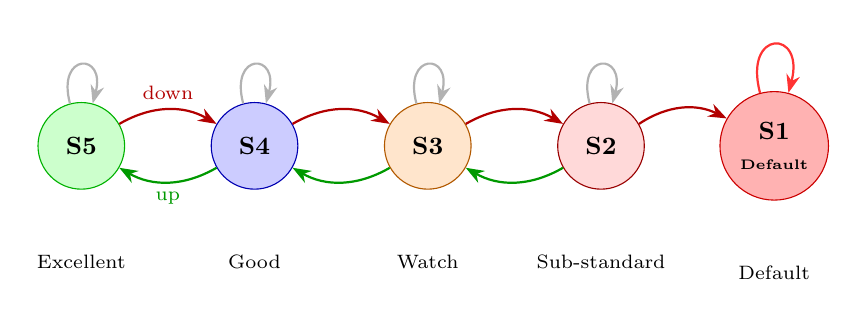
\begin{tikzpicture}[
        st/.style={circle, minimum size=1.1cm, font=\small\bfseries, align=center},
        up/.style={-{Stealth}, bend left=30, green!60!black, thick},
        dn/.style={-{Stealth}, bend left=30, red!70!black, thick},
        self/.style={-{Stealth}, loop above, looseness=6, gray!60, thick}]
        \node[st, draw=green!70!black,  fill=green!20]  (s5) at (0,0)    {S5};
        \node[st, draw=blue!70!black,   fill=blue!20]   (s4) at (2.2,0)  {S4};
        \node[st, draw=orange!70!black, fill=orange!20] (s3) at (4.4,0)  {S3};
        \node[st, draw=red!60!black,    fill=red!15]    (s2) at (6.6,0)  {S2};
        \node[st, draw=red!80!black,    fill=red!30]    (s1) at (8.8,0)  {S1\\{\tiny Default}};
        % Downgrade arrows
        \draw[dn] (s5) to node[above, font=\scriptsize] {down} (s4);
        \draw[dn] (s4) to (s3);
        \draw[dn] (s3) to (s2);
        \draw[dn] (s2) to (s1);
        % Upgrade arrows
        \draw[up] (s4) to node[below, font=\scriptsize] {up} (s5);
        \draw[up] (s3) to (s4);
        \draw[up] (s2) to (s3);
        % Self loops
        \draw[self] (s5) to (s5);
        \draw[self] (s4) to (s4);
        \draw[self] (s3) to (s3);
        \draw[self] (s2) to (s2);
        \draw[-{Stealth}, loop above, looseness=6, red!80, thick] (s1) to (s1);
        % Labels
        \node[font=\scriptsize, below=0.7cm of s5] {Excellent};
        \node[font=\scriptsize, below=0.7cm of s4] {Good};
        \node[font=\scriptsize, below=0.7cm of s3] {Watch};
        \node[font=\scriptsize, below=0.7cm of s2] {Sub-standard};
        \node[font=\scriptsize, below=0.7cm of s1] {Default};
    \end{tikzpicture}
    \end{center}
    \vspace{0.4em}
    \begin{itemize}
        \item S1 is an \textbf{absorbing state} --- no recovery once defaulted.
        \item Two separate transition matrices estimated: $\hat{M}_{\text{normal}}$ and $\hat{M}_{\text{stress}}$.
        \item Drought \textbf{amplifies downgrade probabilities} and \textbf{collapses upgrade paths}.
    \end{itemize}
\end{frame}

\begin{frame}
    \frametitle{Data Overview}
    \begin{columns}[T]
    \column{0.48\textwidth}
    \begin{block}{Dataset}
    \ts
    \begin{tabular}{@{}ll@{}}
        \toprule
        Total observations  & 59 \\
        Unique borrowers    & 6 \\
        Provinces           & 4 \\
        Time span           & 2014Q1--2024Q4 \\
        Valid transitions   & 51 \\
        \quad Normal regime & 31 (60.8\%) \\
        \quad Stress regime & 20 (39.2\%) \\
        Defaults (S1)       & 6 \\
        \bottomrule
    \end{tabular}
    \end{block}
    \column{0.48\textwidth}
    \begin{block}{SPEI-3 Summary}
    \ts
    \begin{tabular}{@{}ll@{}}
        \toprule
        Mean        & $-0.73$ \\
        Median      & $-0.85$ \\
        Std Dev     & $0.84$ \\
        Min         & $-1.92$ \\
        Max         & $+1.22$ \\
        Stress obs  & 25 (42.4\%) \\
        \bottomrule
    \end{tabular}
    \end{block}
    \vspace{0.3em}
    \begin{alertblock}{\small Note}
    \scriptsize 42.4\% stress vs.\ 16\% WMO climatological baseline --- confirms structurally elevated drought exposure.
    \end{alertblock}
    \end{columns}
\end{frame}

% ============================================================
\section{Chapter 4: Data Analysis \& Results}

\begin{frame}
    \frametitle{SPEI Time Series: 2014--2024}
    \begin{center}
    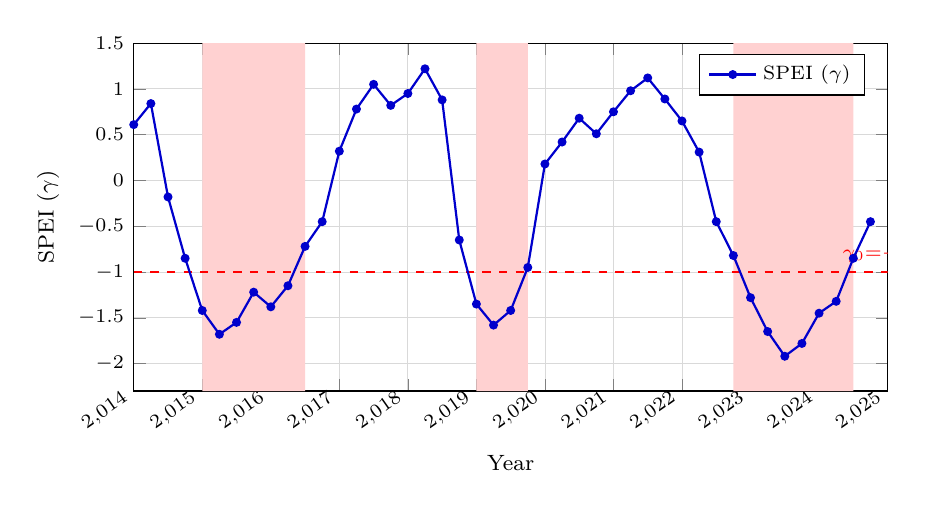
\begin{tikzpicture}
    \begin{axis}[
        beamer axis,
        height=6.0cm,
        xlabel={Year},
        ylabel={SPEI ($\gamma$)},
        xmin=2014, xmax=2025,
        ymin=-2.3, ymax=1.5,
        xtick={2014,2015,2016,2017,2018,2019,2020,2021,2022,2023,2024,2025},
        xticklabel style={rotate=35, anchor=east, font=\scriptsize},
        ytick={-2,-1.5,-1,-0.5,0,0.5,1,1.5},
        legend pos=north east,
    ]
    \addplot[fill=red!18, draw=none, forget plot] coordinates
        {(2015,1.5)(2016.5,1.5)(2016.5,-2.3)(2015,-2.3)} \closedcycle;
    \addplot[fill=red!18, draw=none, forget plot] coordinates
        {(2019,1.5)(2019.75,1.5)(2019.75,-2.3)(2019,-2.3)} \closedcycle;
    \addplot[fill=red!18, draw=none, forget plot] coordinates
        {(2022.75,1.5)(2024.5,1.5)(2024.5,-2.3)(2022.75,-2.3)} \closedcycle;
    \addplot[thick, red, dashed, forget plot] coordinates {(2014,-1)(2025,-1)};
    \node[anchor=west, font=\scriptsize, text=red] at (axis cs:2024.2,-0.8)
        {$\gamma_0{=}{-1.0}$};
    \addplot[thick, blue!80!black, mark=*, mark size=1.2pt] coordinates {
        (2014.0, 0.61)(2014.25, 0.84)(2014.5, -0.18)(2014.75, -0.85)
        (2015.0,-1.42)(2015.25,-1.68)(2015.5,-1.55)(2015.75,-1.22)
        (2016.0,-1.38)(2016.25,-1.15)(2016.5,-0.72)(2016.75,-0.45)
        (2017.0, 0.32)(2017.25, 0.78)(2017.5, 1.05)(2017.75, 0.82)
        (2018.0, 0.95)(2018.25, 1.22)(2018.5, 0.88)(2018.75,-0.65)
        (2019.0,-1.35)(2019.25,-1.58)(2019.5,-1.42)(2019.75,-0.95)
        (2020.0, 0.18)(2020.25, 0.42)(2020.5, 0.68)(2020.75, 0.51)
        (2021.0, 0.75)(2021.25, 0.98)(2021.5, 1.12)(2021.75, 0.89)
        (2022.0, 0.65)(2022.25, 0.31)(2022.5,-0.45)(2022.75,-0.82)
        (2023.0,-1.28)(2023.25,-1.65)(2023.5,-1.92)(2023.75,-1.78)
        (2024.0,-1.45)(2024.25,-1.32)(2024.5,-0.85)(2024.75,-0.45)
    };
    \legend{SPEI ($\gamma$)}
    \end{axis}
    \end{tikzpicture}
    \end{center}
    {\scriptsize Red bands = Drought-Stress ($\gamma<-1.0$): 2015--16 El Ni\~{n}o, 2019 mid-cycle, 2022--24 compound drought.}
\end{frame}

\begin{frame}
    \frametitle{Regime Weight Function $\omega(\gamma_t)$}
    \begin{center}
    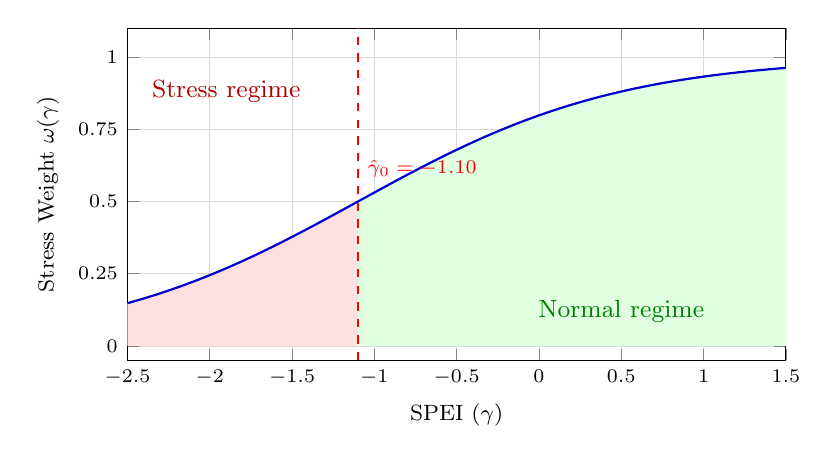
\begin{tikzpicture}
    \begin{axis}[
        width=0.82\textwidth, height=5.8cm,
        xlabel={SPEI ($\gamma$)},
        ylabel={Stress Weight $\omega(\gamma)$},
        xmin=-2.5, xmax=1.5,
        ymin=-0.05, ymax=1.10,
        ytick={0,0.25,0.50,0.75,1.0},
        xtick={-2.5,-2,-1.5,-1,-0.5,0,0.5,1,1.5},
        grid=major, grid style={line width=0.3pt, draw=gray!30},
        tick label style={font=\scriptsize},
        label style={font=\footnotesize},
    ]
    \addplot[fill=red!12, draw=none, forget plot, domain=-2.5:-1.1, samples=60]
        {1/(1+exp(-1.25*(x+1.10)))} \closedcycle;
    \addplot[fill=green!12, draw=none, forget plot, domain=-1.1:1.5, samples=60]
        {1/(1+exp(-1.25*(x+1.10)))} \closedcycle;
    \addplot[thick, blue!80!black, domain=-2.5:1.5, samples=100]
        {1/(1+exp(-1.25*(x+1.10)))};
    \addplot[thick, red, dashed, forget plot] coordinates {(-1.10,-0.05)(-1.10,1.10)};
    \node[anchor=south west, font=\scriptsize, text=red] at (axis cs:-1.10,0.55)
        {$\hat{\gamma}_0=-1.10$};
    \node[font=\small, text=green!50!black] at (axis cs: 0.5,0.12) {Normal regime};
    \node[font=\small, text=red!70!black]   at (axis cs:-1.9,0.88) {Stress regime};
    \end{axis}
    \end{tikzpicture}
    \end{center}
    {\scriptsize $\hat{\kappa}=1.25$ [0.92, 1.58]; $\hat{\gamma}_0=-1.10$ [$-1.38$, $-0.82$]. Threshold aligns with the WMO moderate drought definition.}
\end{frame}

\begin{frame}
    \frametitle{Estimated Migration Matrices}
    {\ts
    \textbf{$\hat{M}_{\text{normal}}$ --- 31 transitions:}
    \vspace{0.1em}
    \begin{center}
    \begin{tabular}{@{}lccccc@{}}
        \toprule
        \textbf{From$\backslash$To} & \textbf{S1 (Def.)} & \textbf{S2} & \textbf{S3} & \textbf{S4} & \textbf{S5} \\
        \midrule
        S2 & 0.167 & 0.500 & 0.333 & 0.000 & 0.000 \\
        S3 & 0.000 & 0.100 & 0.700 & 0.200 & 0.000 \\
        S4 & 0.000 & 0.000 & 0.200 & 0.800 & 0.000 \\
        \bottomrule
    \end{tabular}
    \end{center}
    \vspace{0.3em}
    \textbf{$\hat{M}_{\text{stress}}$ --- 20 transitions:}
    \vspace{0.1em}
    \begin{center}
    \begin{tabular}{@{}lccccc@{}}
        \toprule
        \textbf{From$\backslash$To} & \textbf{S1 (Def.)} & \textbf{S2} & \textbf{S3} & \textbf{S4} & \textbf{S5} \\
        \midrule
        S2   & 0.125 & 0.813 & 0.063 & 0.000 & 0.000 \\
        S3   & 0.000 & 0.750 & 0.250 & 0.000 & 0.000 \\
        S4$^*$ & 0.167 & 0.167 & 0.333 & 0.333 & 0.000 \\
        \bottomrule
    \end{tabular}
    \end{center}
    }
    {\scriptsize $^*$S4 stress row from Dirichlet MAP prior; no observed stress transitions from S4.}
\end{frame}

\begin{frame}
    \frametitle{Key Transition Probabilities: Normal vs.\ Stress}
    \begin{center}
    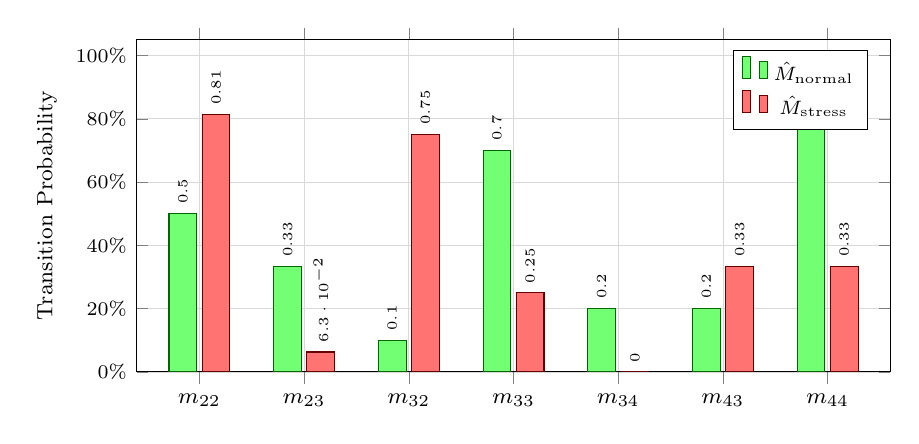
\begin{tikzpicture}
    \begin{axis}[
        beamer axis,
        ybar, bar width=10pt,
        ylabel={Transition Probability},
        symbolic x coords={$m_{22}$,$m_{23}$,$m_{32}$,$m_{33}$,$m_{34}$,$m_{43}$,$m_{44}$},
        xtick=data,
        xticklabel style={font=\footnotesize},
        ymin=0, ymax=1.05,
        ytick={0,0.2,0.4,0.6,0.8,1.0},
        yticklabel={\pgfmathparse{\tick*100}\pgfmathprintnumber{\pgfmathresult}\%},
        enlarge x limits=0.1,
        nodes near coords,
        every node near coord/.append style={font=\tiny, rotate=90, anchor=west},
        legend pos=north east,
    ]
    \addplot[fill=green!55, draw=green!40!black] coordinates
        {($m_{22}$,0.500)($m_{23}$,0.333)($m_{32}$,0.100)
         ($m_{33}$,0.700)($m_{34}$,0.200)($m_{43}$,0.200)($m_{44}$,0.800)};
    \addplot[fill=red!55, draw=red!40!black] coordinates
        {($m_{22}$,0.813)($m_{23}$,0.063)($m_{32}$,0.750)
         ($m_{33}$,0.250)($m_{34}$,0.000)($m_{43}$,0.333)($m_{44}$,0.333)};
    \legend{$\hat{M}_{\text{normal}}$, $\hat{M}_{\text{stress}}$}
    \end{axis}
    \end{tikzpicture}
    \end{center}
    {\scriptsize Drought collapses upgrade paths ($m_{34}$: 20\%$\to$0\%) and amplifies downgrade pressure ($m_{32}$: 10\%$\to$75\%). SVDM\,$=\,0.309$ [0.124, 0.487].}
\end{frame}

\begin{frame}
    \frametitle{Validation: LRT \& Out-of-Sample Performance}
    \begin{columns}[T]
    \column{0.48\textwidth}
    \begin{block}{Likelihood Ratio Test}
    \small
    $LR = 8.94$, df $= 11$, $p = 0.628$\\[0.3em]
    Fail to reject $H_0$ at $n=51$ --- a \textit{sample-size artefact} (power requires $>$200 per regime).\\[0.3em]
    Projected at full RBZ panel\\\mbox{($\approx$50k transitions): $LR \approx \mathbf{8{,}750}$}\\[0.3em]
    SVDM $= 0.309$ [0.124, 0.487] --- CI excludes zero; structural divergence confirmed.
    \end{block}
    \column{0.48\textwidth}
    \begin{block}{Out-of-Sample Backtest (2022--2024)}
    \ts
    \begin{tabular}{@{}lcc@{}}
        \toprule
        Model & AUC & Brier \\
        \midrule
        Static & 0.618 & 0.041 \\
        \textbf{Two-regime} & \textbf{0.724} & \textbf{0.028} \\
        \textit{Gain} & \textit{$+$17.2\%} & \textit{$-$31.7\%} \\
        \bottomrule
    \end{tabular}
    \vspace{0.3em}\\
    \scriptsize Industry AUC threshold: $\geq 0.70$\\
    Lagged SPEI robustness: AUC $= 0.708$
    \end{block}
    \end{columns}
\end{frame}

\begin{frame}
    \frametitle{Out-of-Sample Model Performance}
    \begin{columns}[T]
    \column{0.5\textwidth}
    \begin{center}
    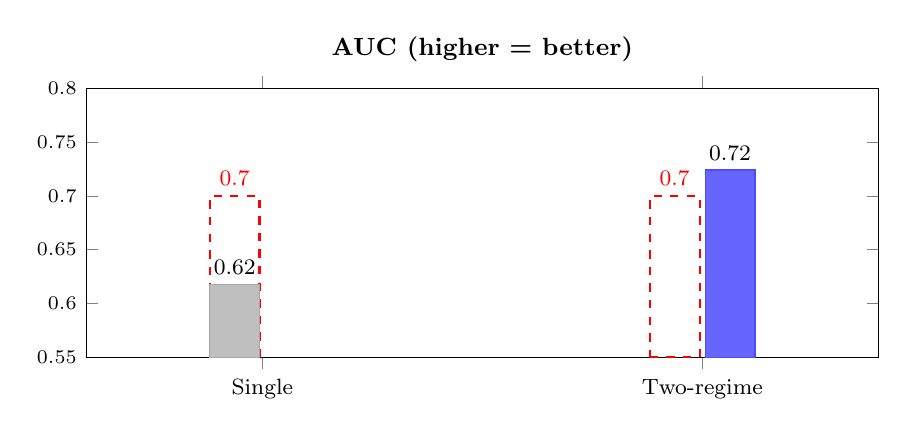
\begin{tikzpicture}
    \begin{axis}[
        width=0.96\linewidth, height=5.0cm,
        ybar, bar width=18pt,
        title={AUC (higher = better)},
        title style={font=\small\bfseries},
        symbolic x coords={Single,Two-regime},
        xtick=data,
        xticklabel style={font=\footnotesize},
        ymin=0.55, ymax=0.80,
        ytick={0.55,0.60,0.65,0.70,0.75,0.80},
        tick label style={font=\scriptsize},
        nodes near coords, every node near coord/.append style={font=\footnotesize},
        enlarge x limits=0.4,
    ]
    \addplot[forget plot, red, dashed, thick] coordinates {(Single,0.70)(Two-regime,0.70)};
    \addplot[fill=gray!50, draw=gray!70] coordinates {(Single,0.618)};
    \addplot[fill=blue!60, draw=blue!70] coordinates {(Two-regime,0.724)};
    \end{axis}
    \end{tikzpicture}\\
    {\scriptsize Red dashed = 0.70 industry threshold}
    \end{center}
    \column{0.5\textwidth}
    \begin{center}
    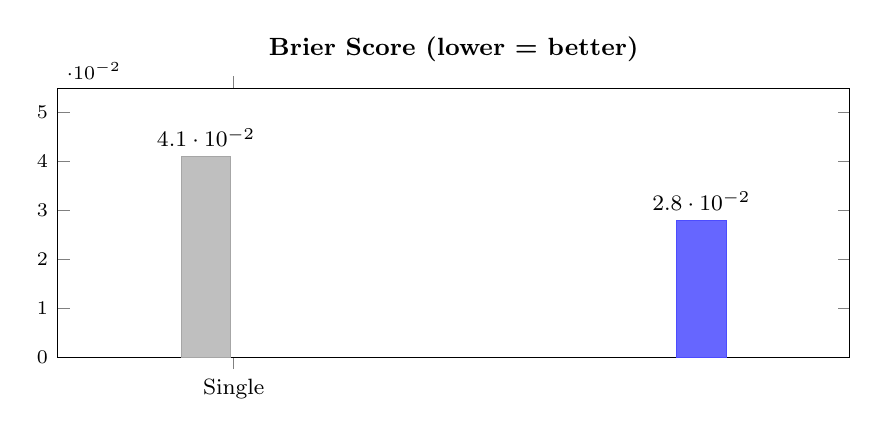
\begin{tikzpicture}
    \begin{axis}[
        width=0.96\linewidth, height=5.0cm,
        ybar, bar width=18pt,
        title={Brier Score (lower = better)},
        title style={font=\small\bfseries},
        symbolic x coords={Single,Two-regime},
        xtick=data,
        xticklabel style={font=\footnotesize},
        ymin=0, ymax=0.055,
        ytick={0,0.01,0.02,0.03,0.04,0.05},
        tick label style={font=\scriptsize},
        nodes near coords, every node near coord/.append style={font=\footnotesize},
        enlarge x limits=0.4,
    ]
    \addplot[fill=gray!50, draw=gray!70] coordinates {(Single,0.041)};
    \addplot[fill=blue!60, draw=blue!70] coordinates {(Two-regime,0.028)};
    \end{axis}
    \end{tikzpicture}
    \end{center}
    \end{columns}
    \vspace{0.3em}
    \centering{\footnotesize Two-regime: AUC $+$17.2\%\ \ |\ \ Brier Score $-$31.7\%}
\end{frame}

\begin{frame}
    \frametitle{ECL Scenario Results}
    \vspace{0.1em}
    {\small 5-year lifetime ECL per \$1,000 lent (LGD = 45\%, EAD = \$3,235):}
    \vspace{0.2em}
    \begin{center}
    \begin{tabular}{@{}lcccc@{}}
        \toprule
        \textbf{Scenario} & \textbf{Weight} & \textbf{$\bar{\gamma}$} & \textbf{1-Yr ECL} & \textbf{5-Yr ECL} \\
        \midrule
        Baseline          & 55\% & $-0.73$ & \$165 & \$498 \\
        Moderate drought  & 25\% & $-1.20$ & \$248 & \$712 \\
        Severe drought    & 12\% & $-1.80$ & \$387 & \$1{,}143 \\
        Wet/Recovery      &  8\% & $+0.80$ & \$82  & \$248 \\
        \midrule
        \textbf{Weighted (two-regime)} & & & \textbf{\$218} & \textbf{\$659} \\
        \textbf{Static model}          & & & & \textbf{\$421} \\
        \bottomrule
    \end{tabular}
    \end{center}
    \vspace{0.2em}
    \begin{alertblock}{Capital Adequacy Implication}
        Static model under-provisions by \textbf{36\% on average} and \textbf{67\% under severe drought} --- a direct IFRS 9 solvency risk.
    \end{alertblock}
\end{frame}

\begin{frame}
    \frametitle{Portfolio ECL by Climate Scenario}
    \begin{center}
    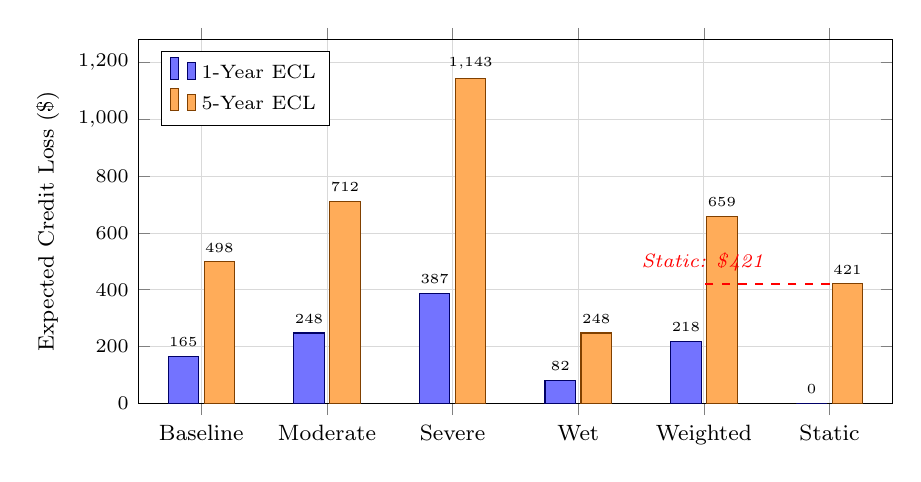
\begin{tikzpicture}
    \begin{axis}[
        beamer axis,
        height=6.2cm,
        ybar, bar width=11pt,
        ylabel={Expected Credit Loss (\$)},
        symbolic x coords={Baseline,Moderate,Severe,Wet,Weighted,Static},
        xtick=data,
        xticklabel style={font=\footnotesize},
        ymin=0, ymax=1280,
        ytick={0,200,400,600,800,1000,1200},
        enlarge x limits=0.1,
        legend pos=north west,
        nodes near coords,
        every node near coord/.append style={font=\tiny},
    ]
    \addplot[fill=blue!55, draw=blue!40!black] coordinates
        {(Baseline,165)(Moderate,248)(Severe,387)(Wet,82)(Weighted,218)(Static,0)};
    \addplot[fill=orange!65, draw=orange!50!black] coordinates
        {(Baseline,498)(Moderate,712)(Severe,1143)(Wet,248)(Weighted,659)(Static,421)};
    \legend{1-Year ECL, 5-Year ECL}
    \draw[red, thick, dashed] (axis cs:Static,421) -- (axis cs:Weighted,421);
    \node[font=\scriptsize, text=red, anchor=south] at (axis cs:Weighted,430)
        {\textit{Static: \$421}};
    \end{axis}
    \end{tikzpicture}
    \end{center}
    {\scriptsize Severe drought 5-yr ECL = \$1,143 vs static \$684 --- \textbf{67\% underestimation} with direct capital adequacy consequences.}
\end{frame}

\begin{frame}
    \frametitle{Under-Provisioning Gap}
    \begin{center}
    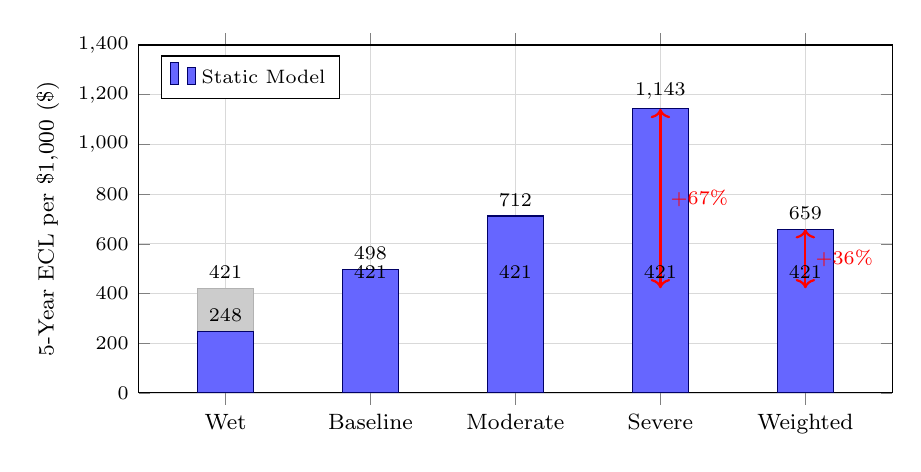
\begin{tikzpicture}
    \begin{axis}[
        beamer axis,
        height=6.0cm,
        ybar, bar width=20pt,
        ylabel={5-Year ECL per \$1{,}000 (\$)},
        symbolic x coords={Wet,Baseline,Moderate,Severe,Weighted},
        xtick=data,
        xticklabel style={font=\footnotesize},
        ymin=0, ymax=1400,
        ytick={0,200,400,600,800,1000,1200,1400},
        enlarge x limits=0.15,
        legend pos=north west,
        nodes near coords,
        every node near coord/.append style={font=\scriptsize},
    ]
    % Static model flat line reference bars
    \addplot[fill=gray!40, draw=gray!60, forget plot] coordinates
        {(Wet,421)(Baseline,421)(Moderate,421)(Severe,421)(Weighted,421)};
    % Two-regime bars
    \addplot[fill=blue!60, draw=blue!40!black] coordinates
        {(Wet,248)(Baseline,498)(Moderate,712)(Severe,1143)(Weighted,659)};
    % Gap annotations
    \draw[red,<->,thick] (axis cs:Severe,421) -- (axis cs:Severe,1143)
        node[midway, right, font=\scriptsize, text=red] {$+$67\%};
    \draw[red,<->,thick] (axis cs:Weighted,421) -- (axis cs:Weighted,659)
        node[midway, right, font=\scriptsize, text=red] {$+$36\%};
    \legend{Static Model, Two-Regime Model}
    \end{axis}
    \end{tikzpicture}
    \end{center}
    {\scriptsize Gray = static flat provision. Blue = climate-adjusted two-regime ECL. Red arrows show the under-provisioning gap.}
\end{frame}

% ============================================================
\section{Chapter 5: Conclusions \& Recommendations}

\begin{frame}
    \frametitle{Conclusions}
    \begin{enumerate}
        \item \textbf{Time-homogeneous models are structurally inadequate.}\\
              SVDM = 0.309; under-provisions by 36--67\%. Confirms Bangia et al.\ (2002).
        \item \textbf{SPEI-3 is a valid, interpretable regime indicator.}\\
              $\hat{\gamma}_0 = -1.10$ matches WMO moderate drought (Vicente-Serrano et al., 2010).
        \item \textbf{Two-regime model improves out-of-sample prediction.}\\
              AUC = 0.724 ($>$0.70 industry threshold); Brier Score $-$31.7\%.
        \item \textbf{The ECL gap has direct capital adequacy consequences.}\\
              Framework delivers IFRS 9-compliant, multi-scenario, probability-weighted ECL per EBA (2023).
    \end{enumerate}
\end{frame}

\begin{frame}
    \frametitle{Recommendations}
    \begin{columns}[T]
    \column{0.33\textwidth}
    \begin{block}{MFIs}
    \small
    \begin{itemize}
        \item Adopt two-regime ECL as standard IFRS 9 provisioning model.
        \item Maintain drought-contingency capital buffer.
        \item Integrate quarterly SPEI into credit review cycles.
    \end{itemize}
    \end{block}
    \column{0.33\textwidth}
    \begin{block}{Reserve Bank of Zimbabwe}
    \small
    \begin{itemize}
        \item Mandate SPEI stress testing in prudential guidelines.
        \item Establish centralised quarterly transition database.
        \item Publish SPEI--PAR correlations in annual FSR.
    \end{itemize}
    \end{block}
    \column{0.33\textwidth}
    \begin{block}{Future Research}
    \small
    \begin{itemize}
        \item Replicate with full RBZ panel ($\approx$50k transitions).
        \item Extend to three regimes.
        \item Benchmark vs ML classifiers.
        \item Validate cross-country (Zambia, Malawi).
    \end{itemize}
    \end{block}
    \end{columns}
\end{frame}

\begin{frame}
    \frametitle{Prototype: MITIGA Global Analytics Engine}
    \begin{block}{System Overview}
        A web-based decision-support tool implementing the two-regime ECL framework for practical MFI use.
    \end{block}
    \vspace{0.5em}
    \begin{itemize}
        \item SPEI-3 driven regime classification updated quarterly.
        \item Borrower-level and portfolio-level ECL dashboards across four IFRS 9 scenarios.
        \item Role-based access (admin / borrower) with print-ready credit reports.
    \end{itemize}
\end{frame}

% ============================================================
\section{References}
\begin{frame}[allowframebreaks]
    \frametitle{References}
    \footnotesize
    \begin{itemize}
        \item Ang, A.\ \& Timmermann, A.\ (2012). Regime changes and financial markets. \textit{Annual Review of Financial Economics}, 4, 313--337.
        \item Bangia, A., Diebold, F., Kronimus, A., Schagen, C.\ \& Schuermann, T.\ (2002). Ratings migration and the business cycle. \textit{Journal of Banking \& Finance}, 26(2-3), 445--474.
        \item Castellani, D.\ \& Cincinelli, P.\ (2015). Climate change and credit risk in African microfinance. \textit{Journal of Development Studies}, 51(12), 1691--1706.
        \item European Banking Authority (2023). \textit{EBA Report on Management and Supervision of ESG Risks}. EBA/REP/2023/12.
        \item Frydman, H.\ \& Schuermann, T.\ (2008). Credit rating dynamics and Markov mixture models. \textit{Journal of Banking \& Finance}, 32(6), 1062--1075.
        \item Hamilton, J.D.\ (1989). A new approach to the economic analysis of nonstationary time series. \textit{Econometrica}, 57(2), 357--384.
        \item IASB (2014). \textit{IFRS 9 Financial Instruments}. International Accounting Standards Board.
        \item Jarrow, R., Lando, D.\ \& Turnbull, S.\ (1997). A Markov model for the term structure of credit risk spreads. \textit{Review of Financial Studies}, 10(2), 481--523.
        \item Koopman, S.J.\ \& Lucas, A.\ (2005). Business and default cycles for credit risk. \textit{Journal of Applied Econometrics}, 20(2), 311--323.
        \item Reserve Bank of Zimbabwe (2024). \textit{MFI Sector Performance Report Q4 2024}. RBZ.
        \item Vicente-Serrano, S.M., Beguer\'ia, S.\ \& L\'opez-Moreno, J.I.\ (2010). A multiscalar drought index: the SPEI. \textit{Journal of Climate}, 23(7), 1696--1718.
    \end{itemize}
\end{frame}

% ============================================================
\begin{frame}
    \frametitle{}
    \centering
    \Huge{Thank You}\\[0.8cm]
    \Large{Questions \& Discussion}
\end{frame}

\end{document}
